\section{Extending your transformation}
\genHeader

At this point, we now have a working TGG to transform a \texttt{Dictionary} into a \texttt{Box} with three \texttt{partition}s, and a \texttt{Box} with exactly three \texttt{Partition}s into a \texttt{Dictionary}. 
The only potential problem is that a learning box with only three partitions may not be the most useful studying tool. 
After all, the more partitions you have, the more practice you'll have with the cards by being quizzed again and again.

A simple strategy would be to allow additional partitions in the box, but to basically ignore them (treat them all as partitions with index greater than two) when transforming to the dictionary. 
To accomplish this we need an extra rule that clearly states how such partitions should be ignored, i.e., be translated without affecting the dictionary. 
We could trivially extend the existing \texttt{BoxToDictionaryRule} by connecting a fourth partition, but what if we wanted a fifth one? A sixth? As you can see, this obviously won't work -- there will always be the potential for a \texttt{n+1}th partition in an \texttt{n}-sized box. 

With a so-called \emph{ignore rule}\define{ignore rule}, we'll handle some source elements and their connecting link variables without creating any new elements in the target domain.
%
Before specifying this ignore rule, however, let's extend the current \texttt{fwd.src.xmi}\footnote{Remember that you should have created this by copying and renaming \texttt{bwd.trg.xmi}.} by adding a new \texttt{Partition} (with \texttt{index} = 3) as depicted in \Cref{fig:ea_extended_fwd_src_xmi}.
Connect the new partition \texttt{partition3}  to \texttt{partition0} via a \texttt{previous} reference, and connect \texttt{partition2} to \texttt{partition3} via a \texttt{next} reference (this is how to extend a learning box).
Create a new \texttt{card} in your new \texttt{partition3} as well.

\begin{figure}[htbp]
\begin{center}
  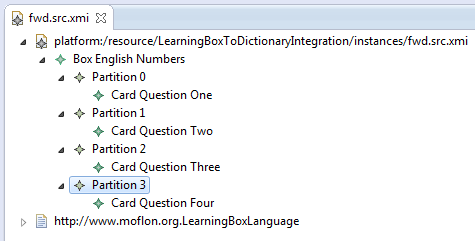
\includegraphics[width=0.6\textwidth]{eclipse_fillFourthPartition}
  \caption{Extended \texttt{fwd.src.xmi}}
  \label{fig:ea_extended_fwd_src_xmi}
\end{center}
\end{figure}


If you run your transformation again, you'll get an error message in the console for the forward direction as our \texttt{fwd.src.xmi} with four \texttt{partition}s cannot be handled with our current TGG.
As this might happen quite often when working on a TGG, let's take some time to understand the message and ``debug'' what went wrong.
The first message in the console is:
\begin{quote}
  \emph{Your TGG LearningBoxLanguageToDictionaryLanguage is not translation locally complete!}
\end{quote}

There are basically two things that can go wrong when transforming a source model to a target model with a TGG-based forward transformation: (1) the input model cannot be completely marked (or ``parsed'', or recognized, etc.)  using TGG rules, and (2) some thing went wrong during the translation of the input model, i.e., when trying to extend the output model.
The first problem is referred to as \emph{input local completeness}, while the second problem is referred to as \emph{translation local completeness}.
The choice of ``input'' vs. ``translation'' should be clear from the above explanation.
The word ``local'' indicates that the transformation is always with respect to a certain match, i.e., a restricted fragment of the models.
If a TGG is ``complete'' then these two problems cannot occur.
This is a nice property to have and getting the compiler to check for this statically is ongoing work. 

What makes things a bit ugly is that our algorithm does not backtrack while searching for a valid rule application sequence as this would make things extremely (exponentially) slow.
The price for this is that we cannot easily differentiate between the case where a TGG rule is simply missing, and the case where a TGG is somehow nasty (requires backtracking) and our algorithm has gotten confused and hit a dead end.
This is why the next message in the console is:
\begin{quote}
\emph{[...] I was unable to translate [...] without backtracking.}
\end{quote}
and not (or slightly more polite isomorphisms thereof):
\begin{quote}
  \emph{You jerk, I don't have a TGG rule to translate this element!!!}
\end{quote}
as you might expect for our concrete example.

After asking you nicely to take a good look at your TGG, the synchroniser tells you exactly where things went wrong:
\begin{quote}
  \emph{I got stuck while trying to extend the following source matches: [CardToEntryRule]}
\end{quote}
That's a bit surprising right?  You probably expected everything to work (as it did before), up to the point where the extra partition turns up and no rule can be found for it.
Well things aren't that straightforward.
To get more information, the synchroniser suggests:
\begin{quote}
  \emph{Set verbose to true in your synchronization helper and re-run to get the exact list of ignored elements.}
\end{quote}
so let's do that and see what happens.

\begin{itemize}
\item[$\blacktriangleright$] Open \texttt{src/org/moflon/tie/Learning\-Box\-Language\-To\-Dictionary\-Lan\-guage\-Trafo.java} and extend the code invoking the forward transformation as follows:
\begin{verbatim}
// Forward Transformation
LearningBoxLan... helper = new LearningBoxLan...Trafo();
helper.setVerbose(true); // <--  add this!
helper.performForward("instances/fwd.src.xmi");
\end{verbatim}
\end{itemize}

If you now rerun the transformation, you'll get a printout of exactly which elements could not be translated at all.
Curiously, this lists include all partitions \emph{and} the box (\texttt{[English Numbers]}).
Although we still do not know why the box and the first three partitions could not be translated using \texttt{BoxToDicationaryRule}, at least we can now understand why the translation failed at \texttt{CardToEntryRule}.
The following happened:
\begin{enumerate}
\item No match could be found for the box and any partition.  
Instead of complaining directly, the algorithm assumes that we do not care about these elements (this is very often the case in practice), so it ignores them and tries to continue with the translation.
\item When translating a card, however, although things look ok on the source side, there is no \texttt{Dictionary} on the target side and the translation fails.
If we would not add the created \texttt{Entry} to the \texttt{Dictionary}, this rule application would have worked! 
\end{enumerate}

OK -- let's now understand why the box was already ignored.

\begin{itemize}
\item[$\blacktriangleright$] Following the four steps in \Cref{fig:dec}, open the generated ecore file in the integration project (Step 1).
This file contains not only the correspondence metamodel, but also all operationalized rules.
Java code for the transformation is generated directly from this file.
\item[$\blacktriangleright$] Under \texttt{Rules/BoxToDictionaryRule/} locate the so called ``isAppriopriate\_FWD...'' method for the TGG rule.
For every TGG rule, three main types of operational rules are derived in each direction:  ``isAppropriate'' methods to check if a match for a rule can be found, ``isApplicable'' to check if this match can be extended to cover all domain, and ``perform'' methods to actually apply the rule in the forward or backward direction.
These methods are all generated as unidirectional programmed graph transformations (story diagrams).
If you want to see how the generated story diagram looks like, go ahead and select the \texttt{Activity} element under the operation (you should get a visualisation as a simple activity diagram).
\item[$\blacktriangleright$] The most important story node in the story diagram (Step 2) is \texttt{test core match and DEC} (all others are more or less bookkeeping and technical stuff).
DEC stands for ``Dangling Edge Condition'' and represents a lookahead for the algorithm.
The basic idea is to check for edges that would be impossible to translate if this rule is applied at this location.
This can be checked for statically and the result of this DEC analyis is embedded in the transformation as simple Negative Application Conditions (NACs). 
Go ahead and select the story pattern (Step~3).
Note that it was derived directly from the TGG rule and, in this sense, \emph{is still a} TGG rule (at least according to the metamodel).
You should see an object diagram representing the rule.
Note that black means context, while blue means negative (it should not be possible to extend a match to cover any of these elements).

\item[$\blacktriangleright$] In our case, there are quite a few edges that would be left (in this sense) dangling.
An example is shown as Step~4 in \Cref{fig:dec}:  if the box has any other contained partition apart from the 3 matched in this rule, then it is clear that this extra edge cannot be translated with any other rule in the current TGG.
It would thus be dangling and therefore blocks the application of this rule.
Another example would be a next edge going out from \texttt{partition2}.
Can you locate the NAC for this edge?
\end{itemize}

\begin{figure}[htbp]
\begin{center}
  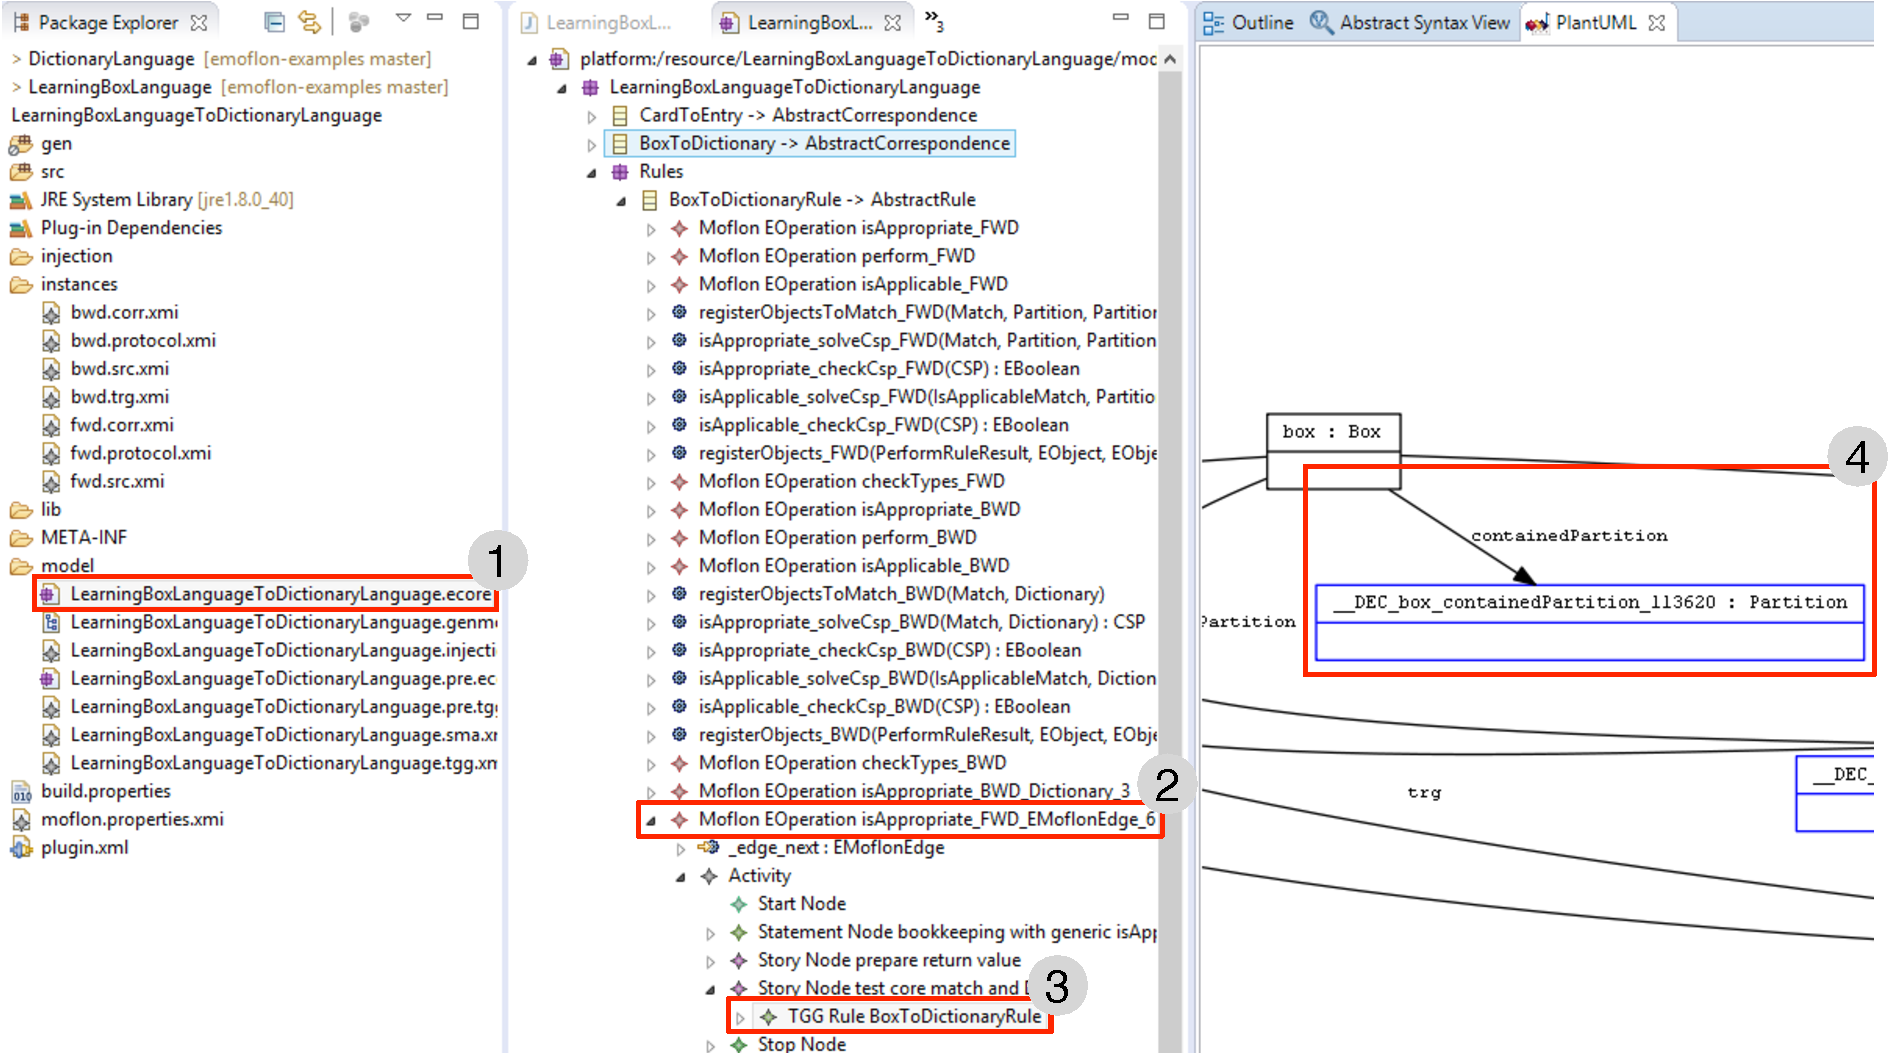
\includegraphics[width=\textwidth]{explanationDEC}
  \caption{Understanding the Dangling Edge Condition}
  \label{fig:dec}
\end{center}
\end{figure}

DEC is a great help when it comes to avoiding dead ends without using backtracking, but in our case where the TGG is actually missing a rule, it only postpones the problem and makes it a bit challenging to understand what went wrong.
On the bright side we took the chance to dig in a bit right?
If you ever have problems understanding why a certain match was not collected, feel free to debug the generated Java code directly if looking at the visualisation does not help (as we did here).
Just place breakpoints as usual and run the transformation in debug modus.
The generated code is quite readable (at least after a week of practice -- haha!).

\newpage
\hypertarget{allCards vis}{}
\subsection{AllOtherPartitionsRule}
\genHeader

\begin{itemize}

\item[$\blacktriangleright$] Create a new rule \texttt{AllOtherPartitionsRule}, and complete it according to \Cref{fig:ea_AllOtherPartitionsRuleComplete}.


\begin{figure}[htbp]
\begin{center}
  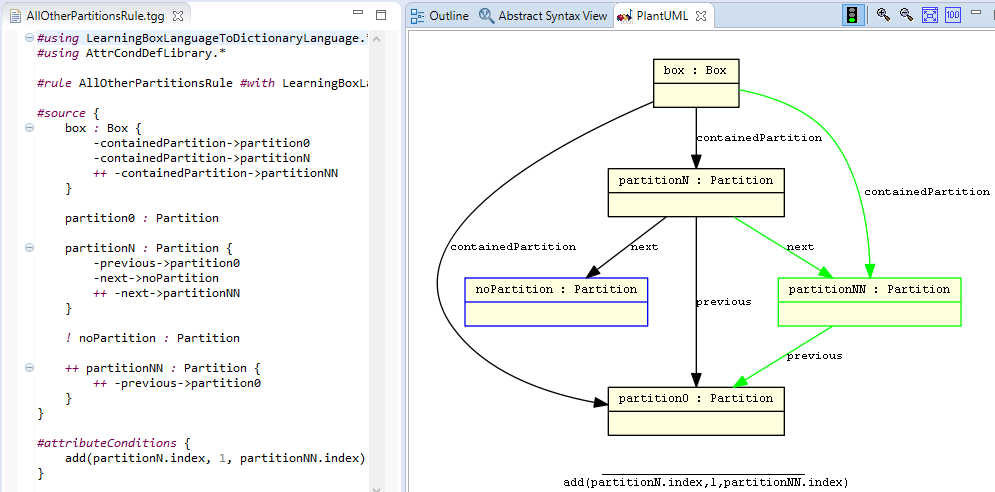
\includegraphics[width=\textwidth]{ea_AllOtherPartitionsRule}
  \caption{The completed \texttt{AllOtherPartitionsRule}}
  \label{fig:ea_AllOtherPartitionsRuleComplete}
\end{center}
\end{figure}

\item[$\blacktriangleright$] As you can see, this rule doesn't assume to know the final \texttt{partition} in the transformation. 
It matches the \texttt{n}th partition as the partition without any next partition, then connects a new \texttt{n+1}th partition to \texttt{n} and \texttt{partition0} (clear as every partitions previous is \texttt{partition0}).
Note that TGG transformations assume that the models are valid, i.e., have the expected structure (in our case meaning that the learning box is correctly ``wired'').\footnote{This should actually be formalised with a set of metamodel constraints that must be checked before a transformation is run, but we've omitted this here to simplify things.}  
Remember that ``blue'' means ``negative''.

\item[$\blacktriangleright$] Generate code for your improved TGG and re-run the transformation. 
It should work now without any error message.
Inspect the protocol to understand what happened.

\item[$\blacktriangleright$] Go ahead and add as many \texttt{partition}s and \texttt{card}s as you like to your model instance.
Your TGG is now also able to handle a \texttt{box} with any number of \texttt{partition}s beautifully.
For five partitions all with cards, the protocol gets quite interesting and is no longer a flat tree.
Try it out! 

\end{itemize}



%%% Local Variables: 
%%% mode: latex
%%% TeX-master: "../src/TGG_mainFile"
%%% End: 




%%% Local Variables: 
%%% mode: latex
%%% TeX-master: "../src/TGG_mainFile"
%%% End: 